% =====================================================================
% Results and analysis (LBF study). Needs: graphicx, booktabs, tabularx,
% multirow, natbib, and the \ci macro defined in main.tex.
% =====================================================================
\section{Results and Analysis}
\label{sec:results}

\paragraph{Setup.}
We evaluate QMIX~\citep{qmix}, QPLEX~\citep{wang2021qplex}, MAPPO~\citep{yu2022mappo},
MACPF~\citep{macpf}, and the adaptive TD($\lambda$) (ATD) variants of QMIX, QPLEX and
MAPPO~\citep{deng2026adaptive}. The evaluation uses the seven Level-Based Foraging (LBF) tasks
of the benchmark of Papoudakis et al.~\citep{test} (arXiv:2006.07869v4, Table~3).
To separate the effect of \emph{adapting} $\lambda$ from the effect of using $\lambda$-returns
at all, we also run fixed-$\lambda$ controls:
\begin{itemize}
  \item QMIX and QPLEX with $\lambda=0.4$, the \texttt{td\_lambda} of the ATD paper's own
        baselines;
  \item MAPPO whose critic regresses on $\lambda$-returns with $\lambda=0.95$.
\end{itemize}
The protocol follows the benchmark:
\begin{itemize}
  \item \textbf{Budget.} Off-policy methods train for 2M environment steps, MAPPO for 20M.
  \item \textbf{Evaluation.} 41 evaluations, each the mean return of 100 episodes.
  \item \textbf{Maximum return.} The evaluation step with the highest mean over seeds, reported
        as mean $\pm$ 95\% CI over seeds at that step.
  \item \textbf{Average return.} The mean over all 41 evaluations.
\end{itemize}
We use 3 seeds (the benchmark uses 5), so 210 runs in total. Returns are normalised so that
collecting every item gives 1. Appendix~\ref{app:hyper} lists every hyper-parameter and its
source.

% ---------------------------------------------------------------------
\subsection{Comparison with the benchmark}

\begin{table}[t]
\centering
\caption{\textbf{Maximum returns} (mean $\pm$ 95\% CI) on the seven LBF tasks: our runs (3 seeds)
against the values Papoudakis et al.\ report for the same algorithm and task (Table~3 of
arXiv:2006.07869v4; 5 seeds, parameter sharing). The benchmark does not include QPLEX or MACPF.
\textsuperscript{$\ast$}: tasks where our QMIX is clearly below the paper.}
\label{tab:max}
\small
\setlength{\tabcolsep}{4pt}
\begin{tabular}{l cc cc c c}
\toprule
 & \multicolumn{2}{c}{QMIX} & \multicolumn{2}{c}{MAPPO} & QPLEX & MACPF \\
\cmidrule(lr){2-3}\cmidrule(lr){4-5}\cmidrule(lr){6-6}\cmidrule(lr){7-7}
Task & ours & paper & ours & paper & ours & ours \\
\midrule
8x8-2p-2f-c\textsuperscript{$\ast$} & 0.48\ci{0.05} & 0.96\ci{0.07} & 1.00\ci{0.00} & 1.00\ci{0.00} & 1.00\ci{0.00} & 0.23\ci{0.38} \\
8x8-2p-2f-2s-c                      & 0.99\ci{0.01} & 1.00\ci{0.00} & 0.86\ci{0.12} & 0.85\ci{0.06} & 1.00\ci{0.00} & 0.01\ci{0.06} \\
10x10-3p-3f\textsuperscript{$\ast$} & 0.23\ci{0.10} & 0.84\ci{0.08} & 0.99\ci{0.02} & 0.99\ci{0.01} & 0.18\ci{0.14} & 0.10\ci{0.21} \\
10x10-3p-3f-2s                      & 0.88\ci{0.06} & 0.90\ci{0.01} & 0.74\ci{0.14} & 0.72\ci{0.03} & 0.92\ci{0.03} & 0.09\ci{0.16} \\
15x15-3p-5f                         & 0.06\ci{0.02} & 0.09\ci{0.04} & 0.78\ci{0.05} & 0.77\ci{0.02} & 0.02\ci{0.02} & 0.04\ci{0.04} \\
15x15-4p-3f                         & 0.10\ci{0.06} & 0.15\ci{0.06} & 0.97\ci{0.01} & 0.96\ci{0.02} & 0.05\ci{0.06} & 0.04\ci{0.10} \\
15x15-4p-5f\textsuperscript{$\ast$} & 0.08\ci{0.03} & 0.25\ci{0.09} & 0.83\ci{0.13} & 0.70\ci{0.25} & 0.04\ci{0.05} & 0.08\ci{0.22} \\
\bottomrule
\end{tabular}
\end{table}

\begin{table}[t]
\centering
\caption{\textbf{Average returns} over all 41 evaluations (mean $\pm$ 95\% CI), ours against
Table~6 of the benchmark (arXiv:2006.07869v4).}
\label{tab:avg}
\small
\setlength{\tabcolsep}{4pt}
\begin{tabular}{l cc cc c c}
\toprule
 & \multicolumn{2}{c}{QMIX} & \multicolumn{2}{c}{MAPPO} & QPLEX & MACPF \\
\cmidrule(lr){2-3}\cmidrule(lr){4-5}\cmidrule(lr){6-6}\cmidrule(lr){7-7}
Task & ours & paper & ours & paper & ours & ours \\
\midrule
8x8-2p-2f-c    & 0.24\ci{0.12} & 0.39\ci{0.10} & 0.95\ci{0.02} & 0.95\ci{0.01} & 0.64\ci{0.04} & 0.10\ci{0.15} \\
8x8-2p-2f-2s-c & 0.56\ci{0.15} & 0.77\ci{0.03} & 0.74\ci{0.02} & 0.77\ci{0.02} & 0.67\ci{0.10} & 0.00\ci{0.00} \\
10x10-3p-3f    & 0.11\ci{0.06} & 0.32\ci{0.07} & 0.91\ci{0.04} & 0.91\ci{0.01} & 0.10\ci{0.10} & 0.04\ci{0.07} \\
10x10-3p-3f-2s & 0.59\ci{0.06} & 0.67\ci{0.01} & 0.65\ci{0.03} & 0.66\ci{0.01} & 0.62\ci{0.09} & 0.06\ci{0.04} \\
15x15-3p-5f    & 0.03\ci{0.02} & 0.04\ci{0.01} & 0.47\ci{0.06} & 0.43\ci{0.09} & 0.01\ci{0.00} & 0.02\ci{0.01} \\
15x15-4p-3f    & 0.06\ci{0.02} & 0.08\ci{0.01} & 0.81\ci{0.08} & 0.79\ci{0.03} & 0.02\ci{0.02} & 0.02\ci{0.03} \\
15x15-4p-5f    & 0.06\ci{0.02} & 0.09\ci{0.02} & 0.42\ci{0.20} & 0.39\ci{0.14} & 0.02\ci{0.01} & 0.04\ci{0.09} \\
\bottomrule
\end{tabular}
\end{table}

\begin{figure}[t]
\centering
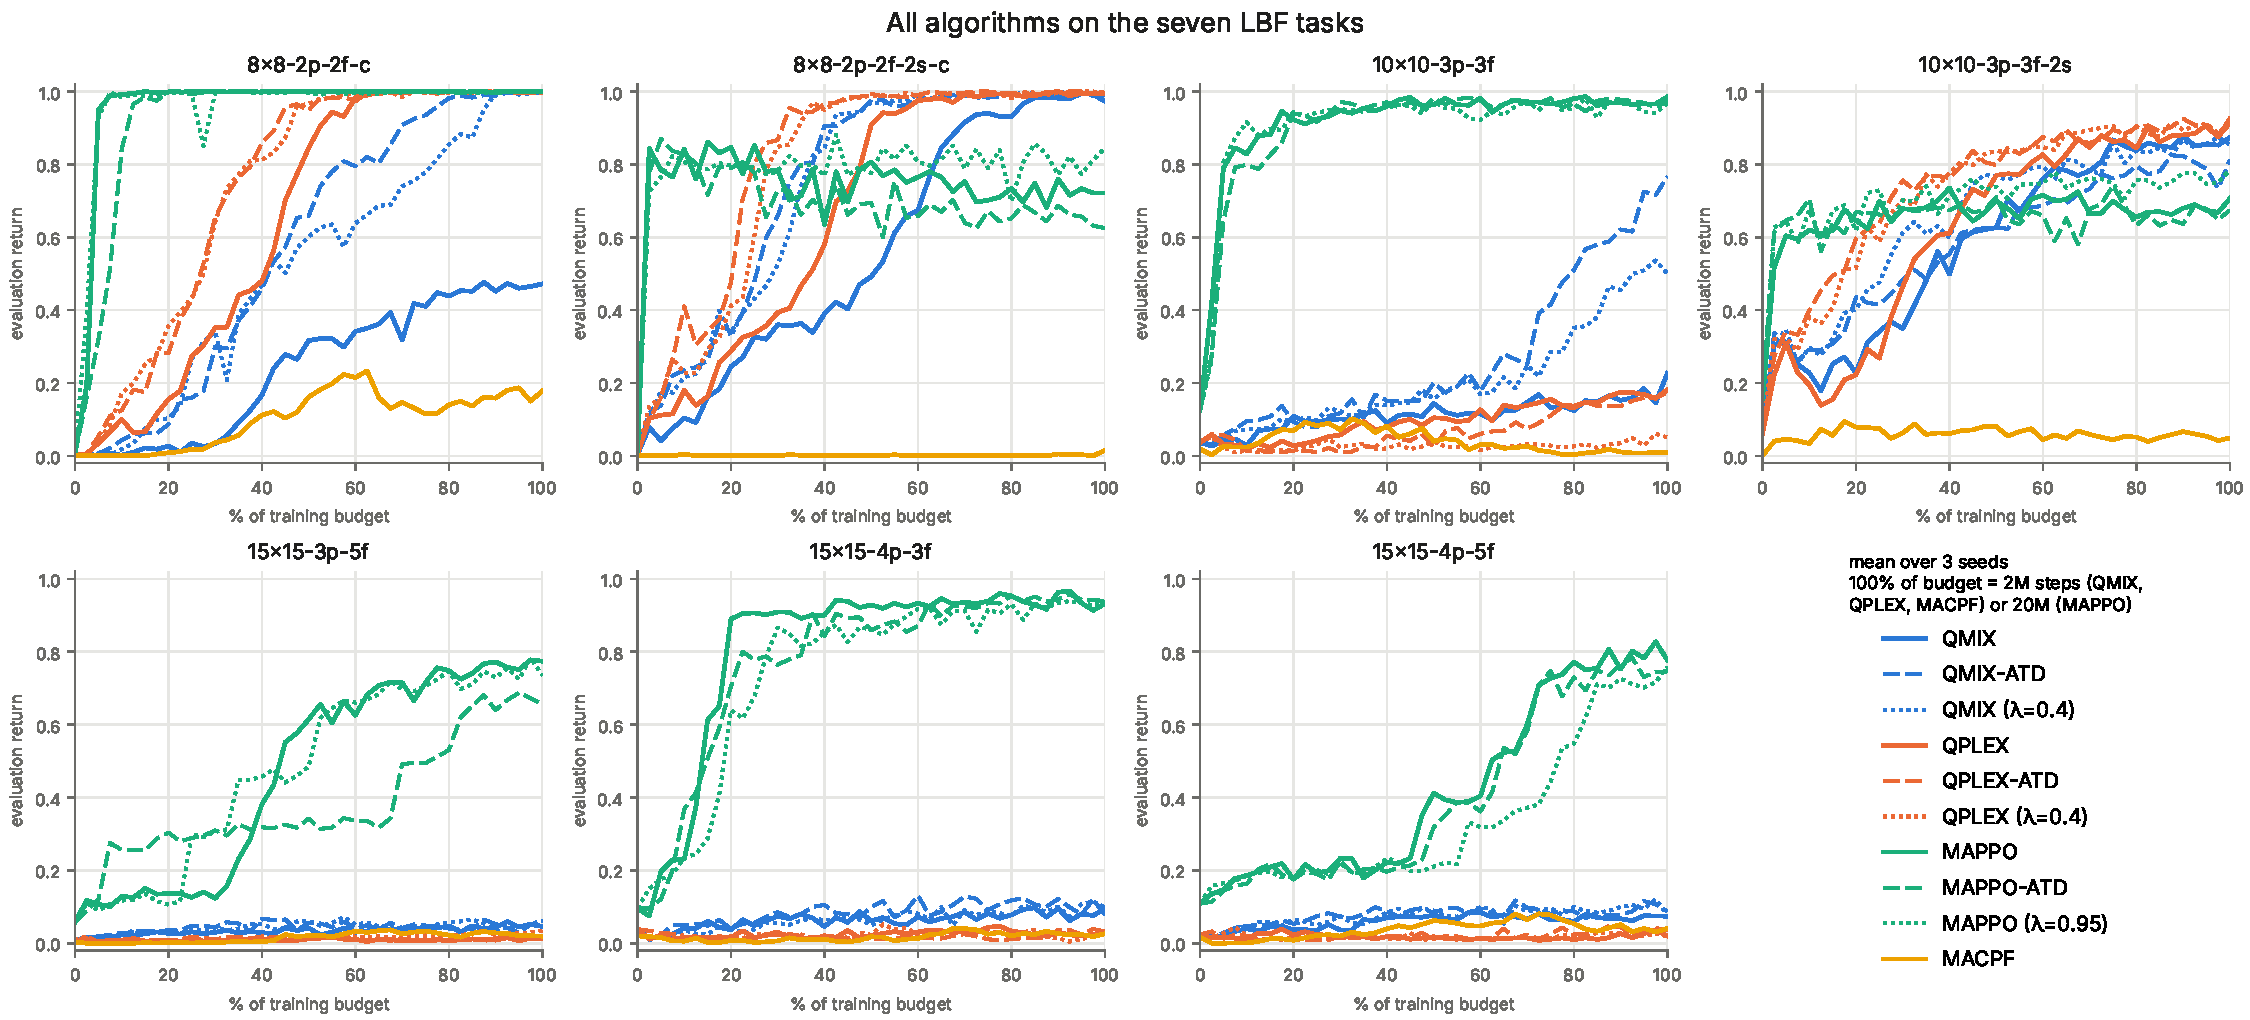
\includegraphics[width=\textwidth]{curves_all.pdf}
\caption{Evaluation return of all ten algorithms on the seven LBF tasks (mean over 3 seeds).
Colour encodes the base algorithm and line style the variant: solid is the base, dashed is ATD,
dotted is fixed $\lambda$. The $x$-axis is the fraction of each algorithm's own budget: 2M steps
for QMIX, QPLEX and MACPF, 20M for MAPPO. At equal $x$, MAPPO has therefore seen ten times more
data. Confidence bands are omitted for legibility; Fig.~\ref{fig:qmix} shows them for the QMIX
family.}
\label{fig:all}
\end{figure}

Tables~\ref{tab:max} and~\ref{tab:avg} and Fig.~\ref{fig:all} summarise the main results.

\textbf{MAPPO reproduces the benchmark.} On every task our maximum and average returns lie within,
or overlap, the paper's confidence intervals. MAPPO is also the only method that makes progress
on the three $15\times15$ tasks.

\textbf{QMIX reproduces the benchmark on four of seven tasks.} It matches on 8x8-2p-2f-2s-c,
10x10-3p-3f-2s, 15x15-3p-5f and 15x15-4p-3f, and is clearly lower on three tasks:
\begin{itemize}
  \item 8x8-2p-2f-c: 0.48 vs.\ 0.96. All three seeds plateau near 0.5, i.e.\ one of the two items,
        so the gap is systematic rather than seed noise.
  \item 10x10-3p-3f: 0.23 vs.\ 0.84.
  \item 15x15-4p-5f: 0.08 vs.\ 0.25.
\end{itemize}
Its average returns are lower than the paper's on the small tasks, i.e.\ it also learns more
slowly. We use the paper's tuned LBF hyper-parameters and did not find the cause. The same QMIX
trained on $\lambda$-returns ($\lambda=0.4$ or ATD; Table~\ref{tab:atd}) reaches 1.00 on
8x8-2p-2f-c and 0.54--0.77 on 10x10-3p-3f. This suggests the gap comes from the 1-step target
propagating the sparse reward too slowly, which an implementation detail not fixed by the paper
could make worse. Papoudakis et al.\ themselves flag their QMIX result on 8x8-2p-2f-c as
high-variance.

\textbf{QPLEX} uses QMIX's training settings, so it differs from QMIX only in the mixer. It is the
best value-based method on three of the four small tasks, and fails on 10x10-3p-3f and on all
$15\times15$ tasks, as QMIX does. \textbf{MACPF} uses its paper's StarCraft settings and was not
tuned for LBF; it does not learn LBF (best: 0.23\ci{0.38}).

% ---------------------------------------------------------------------
\subsection{Adaptive vs.\ fixed $\lambda$}

\begin{table}[t]
\centering
\caption{\textbf{Maximum returns} (mean $\pm$ 95\% CI over 3 seeds) of each base learner, its ATD
variant and its fixed-$\lambda$ control.}
\label{tab:atd}
\scriptsize
\setlength{\tabcolsep}{2.5pt}
\resizebox{\textwidth}{!}{%
\begin{tabular}{l ccc ccc ccc}
\toprule
 & \multicolumn{3}{c}{QMIX} & \multicolumn{3}{c}{QPLEX} & \multicolumn{3}{c}{MAPPO} \\
\cmidrule(lr){2-4}\cmidrule(lr){5-7}\cmidrule(lr){8-10}
Task & base & ATD & $\lambda{=}0.4$ & base & ATD & $\lambda{=}0.4$ & base & ATD & $\lambda{=}0.95$ \\
\midrule
8x8-2p-2f-c    & 0.48\ci{0.05} & 1.00\ci{0.00} & 1.00\ci{0.00} & 1.00\ci{0.00} & 1.00\ci{0.00} & 1.00\ci{0.00} & 1.00\ci{0.00} & 1.00\ci{0.00} & 1.00\ci{0.00} \\
8x8-2p-2f-2s-c & 0.99\ci{0.01} & 1.00\ci{0.01} & 1.00\ci{0.00} & 1.00\ci{0.00} & 1.00\ci{0.00} & 1.00\ci{0.00} & 0.86\ci{0.12} & 0.87\ci{0.16} & 0.88\ci{0.04} \\
10x10-3p-3f    & 0.23\ci{0.10} & 0.77\ci{0.30} & 0.54\ci{0.48} & 0.18\ci{0.14} & 0.17\ci{0.13} & 0.06\ci{0.11} & 0.99\ci{0.02} & 0.98\ci{0.02} & 0.98\ci{0.02} \\
10x10-3p-3f-2s & 0.88\ci{0.06} & 0.82\ci{0.09} & 0.87\ci{0.11} & 0.92\ci{0.03} & 0.93\ci{0.02} & 0.92\ci{0.03} & 0.74\ci{0.14} & 0.74\ci{0.07} & 0.78\ci{0.08} \\
15x15-3p-5f    & 0.06\ci{0.02} & 0.07\ci{0.03} & 0.07\ci{0.03} & 0.02\ci{0.02} & 0.02\ci{0.04} & 0.03\ci{0.08} & 0.78\ci{0.05} & 0.69\ci{0.16} & 0.78\ci{0.12} \\
15x15-4p-3f    & 0.10\ci{0.06} & 0.13\ci{0.02} & 0.11\ci{0.02} & 0.05\ci{0.06} & 0.04\ci{0.05} & 0.05\ci{0.11} & 0.97\ci{0.01} & 0.96\ci{0.06} & 0.94\ci{0.11} \\
15x15-4p-5f    & 0.08\ci{0.03} & 0.12\ci{0.08} & 0.12\ci{0.07} & 0.04\ci{0.05} & 0.05\ci{0.06} & 0.04\ci{0.08} & 0.83\ci{0.13} & 0.78\ci{0.15} & 0.76\ci{0.21} \\
\bottomrule
\end{tabular}}
\end{table}

\begin{figure}[t]
\centering
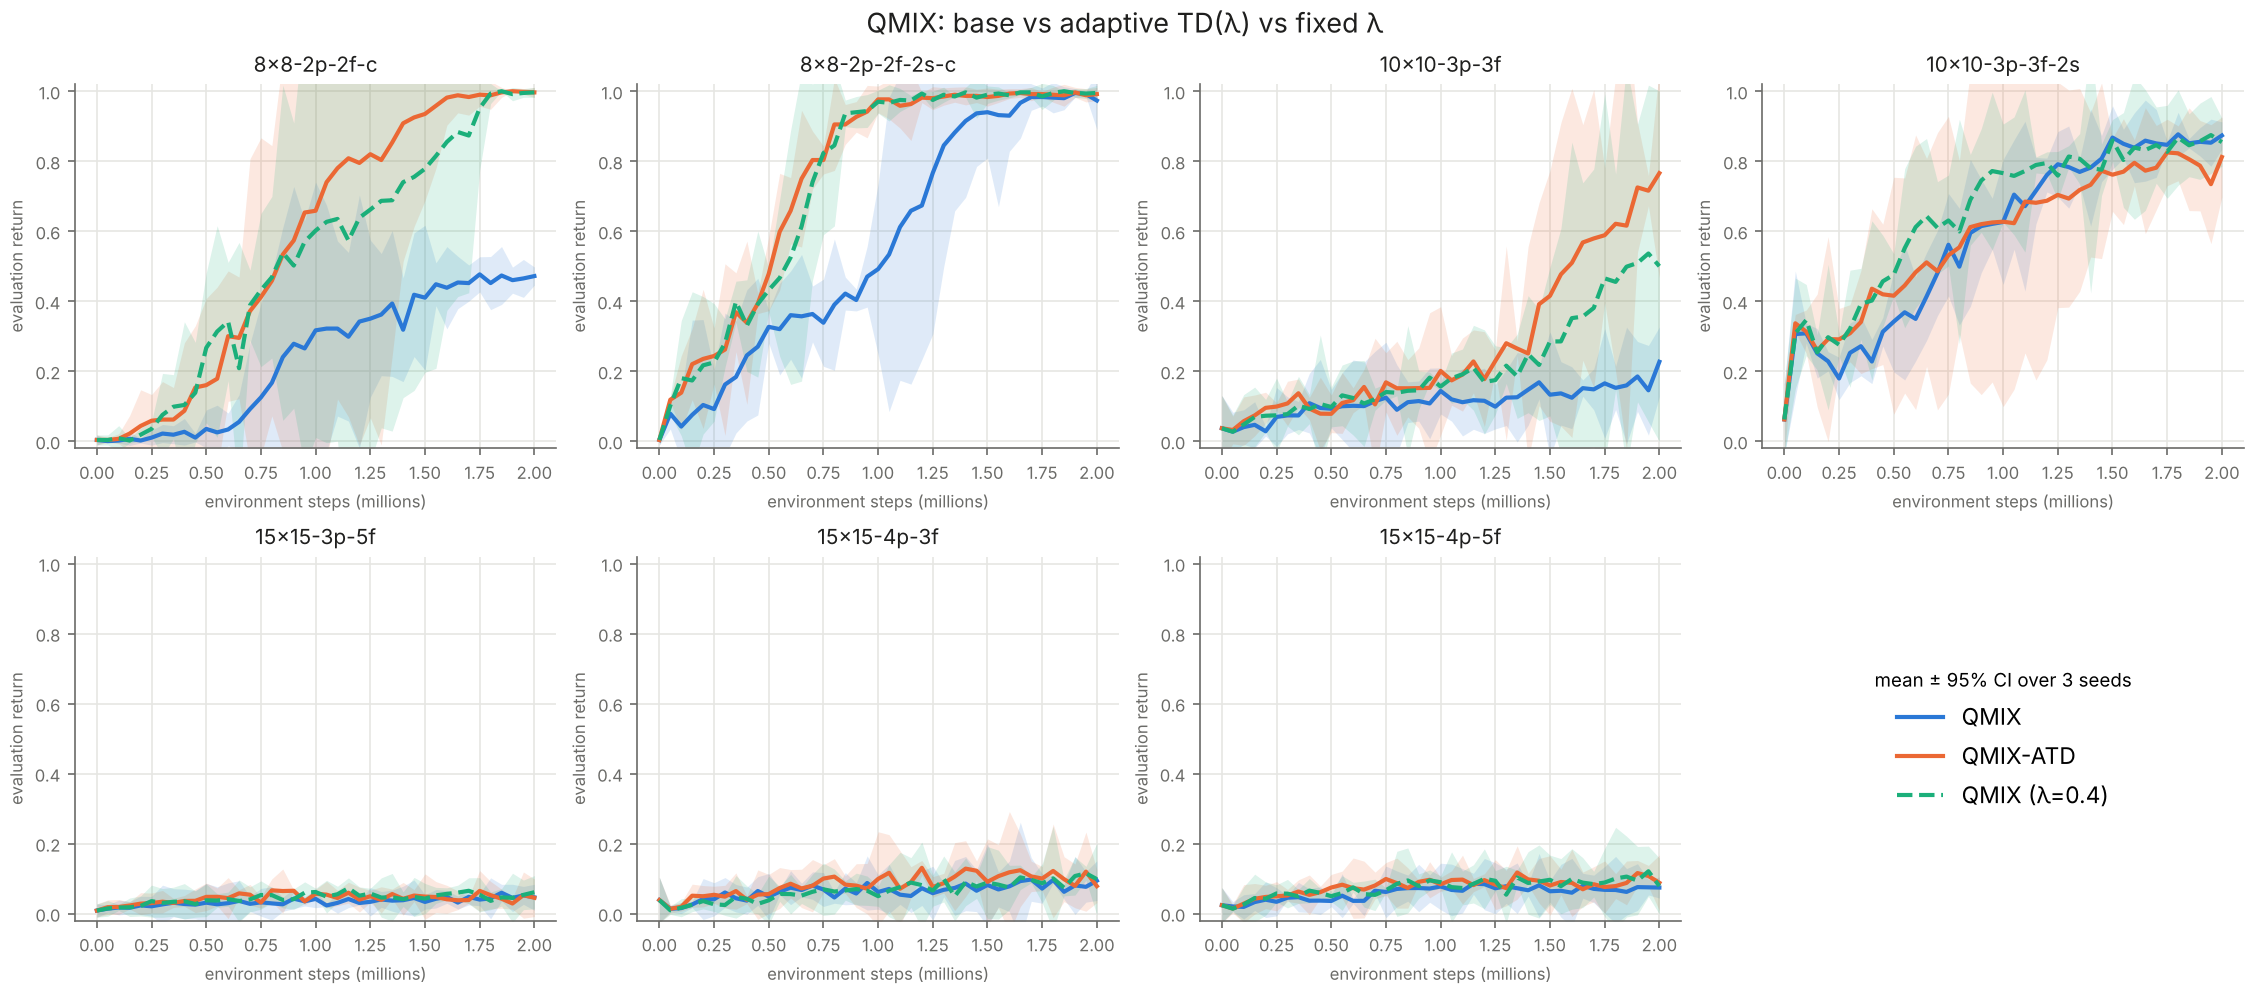
\includegraphics[width=\textwidth]{curves_qmix_atd.png}
\caption{QMIX, QMIX-ATD and QMIX with fixed $\lambda=0.4$ (mean $\pm$ 95\% CI over 3 seeds).
The fixed-$\lambda$ control tracks ATD on every task.}
\label{fig:qmix}
\end{figure}

Table~\ref{tab:atd} and Fig.~\ref{fig:qmix} compare each base learner with its two $\lambda$
variants.
\begin{itemize}
  \item \textbf{QMIX.} ATD improves over 1-step targets on 8x8-2p-2f-c (0.48$\to$1.00) and
        10x10-3p-3f (0.23$\to$0.77). It also improves average return on the two 8x8 tasks
        (0.24$\to$0.57 and 0.56$\to$0.75). The fixed $\lambda=0.4$ control obtains the same
        gains: its confidence intervals overlap ATD's on every task.
  \item \textbf{QPLEX.} The same pattern holds in average return, e.g.\ 0.67$\to$0.81 for ATD
        and 0.79 for $\lambda=0.4$ on 8x8-2p-2f-2s-c.
  \item \textbf{MAPPO.} The critic already uses 5-step returns, and the base, ATD and
        $\lambda=0.95$ are statistically indistinguishable on all tasks.
\end{itemize}
In short, the benefit comes from using $\lambda$-returns at all; adapting $\lambda$ per
state-action pair adds nothing measurable here. Section~\ref{sec:lambda} explains why.

% ---------------------------------------------------------------------
\subsection{Why the adaptive $\lambda$ stays constant}
\label{sec:lambda}

\begin{figure}[t]
\centering
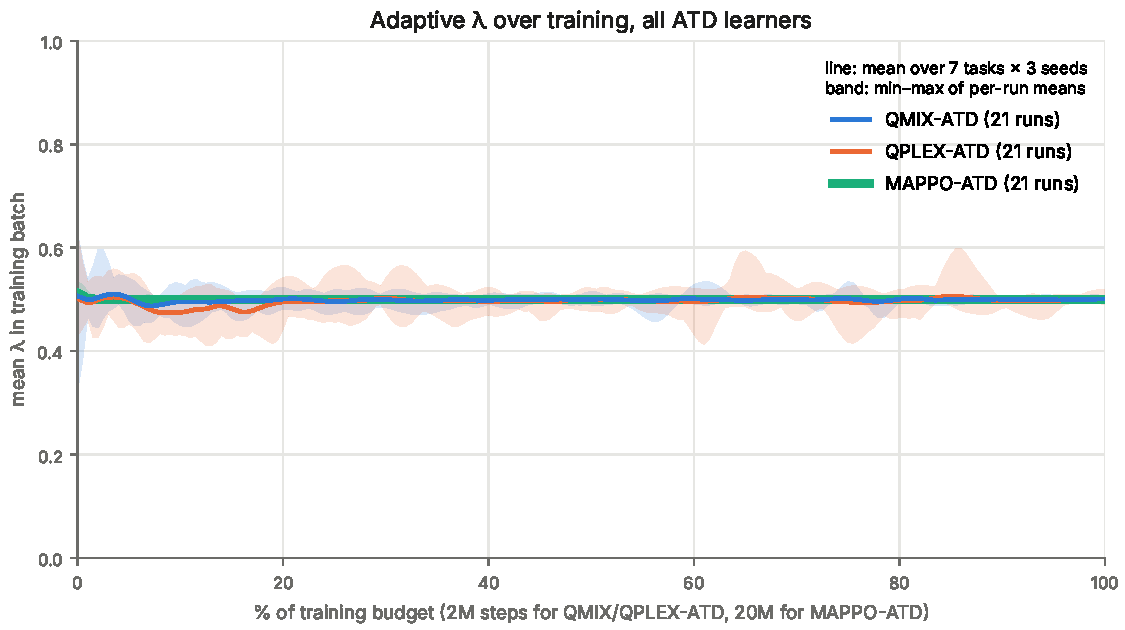
\includegraphics[width=0.8\textwidth]{lambda_all.pdf}
\caption{Mean $\lambda$ in each training batch for the three ATD learners, against the fraction
of each learner's budget. Lines are the mean over 7 tasks $\times$ 3 seeds; bands are the range
of the per-run means. The dotted line is $\lambda=0.5$.}
\label{fig:lambda}
\end{figure}

\begin{figure}[t]
\centering
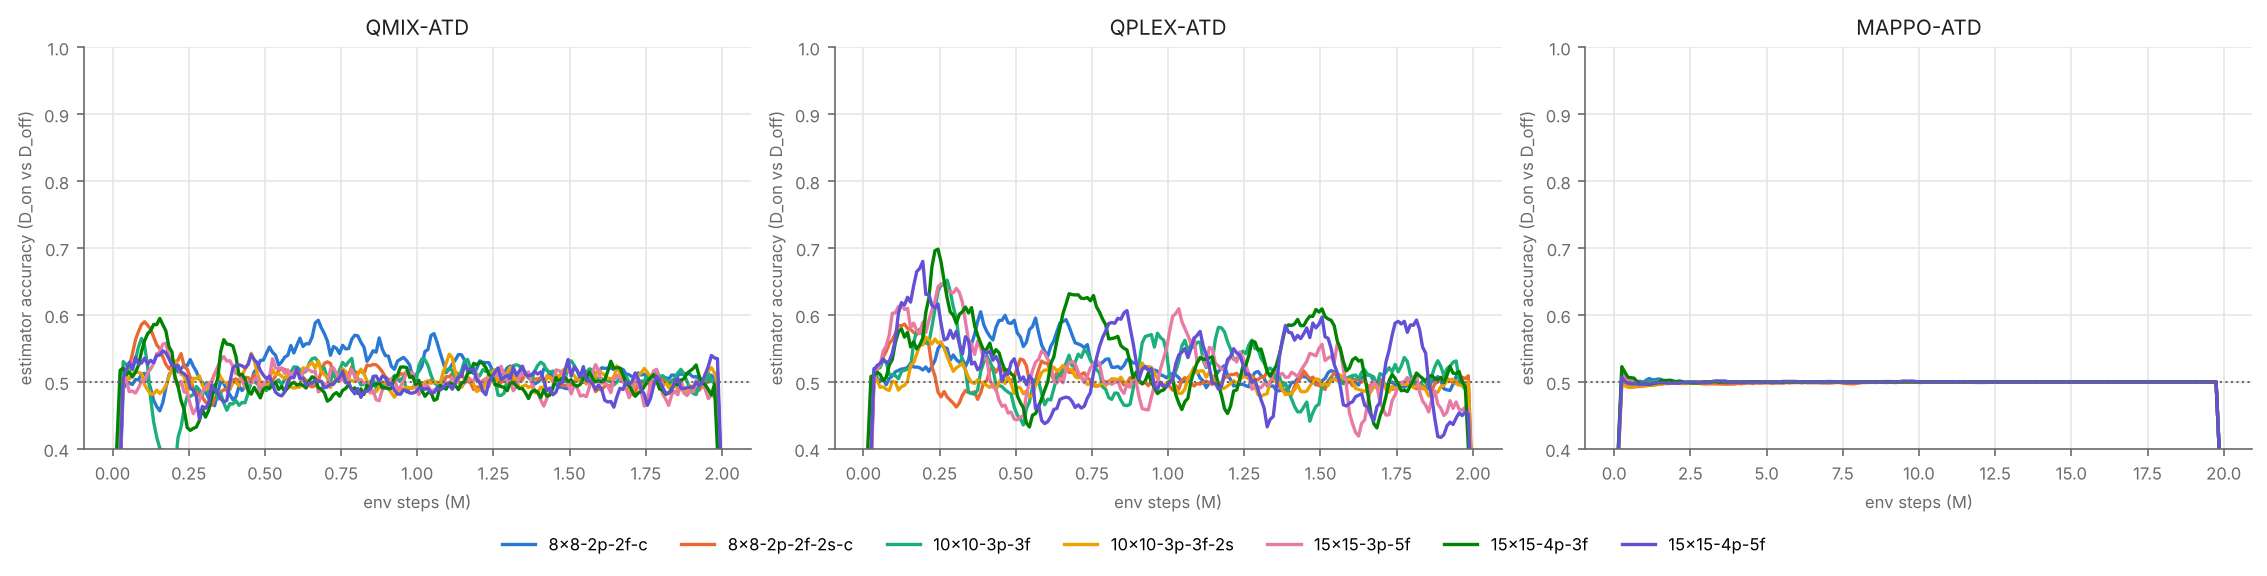
\includegraphics[width=\textwidth]{atd_estimator_accuracy.png}
\caption{Accuracy of the ATD estimator at classifying its training samples as $\mathcal{D}_{on}$
or $\mathcal{D}_{off}$, per task (mean over seeds). The dotted line is chance (0.5).}
\label{fig:acc}
\end{figure}

Fig.~\ref{fig:lambda} shows that $\lambda$ stays at $\approx 0.5$ throughout training for all
three ATD learners on all seven tasks. The spread within a batch is also tiny. Over the second
half of training, the mean per-batch standard deviation of $\lambda$ is 0.018 (QMIX-ATD), 0.021
(QPLEX-ATD) and $<10^{-4}$ (MAPPO-ATD). The 10th--90th percentiles are 0.48--0.52, 0.47--0.53 and
0.500--0.500. So $\lambda$ is constant not only on average but for every state-action pair.

\paragraph{Mechanism.} ATD sets $\lambda(s,a)=\sigma\bigl(\omega(s,a)\bigr)$. The network $\omega$
is trained with a binary cross-entropy that labels samples from a recent buffer
$\mathcal{D}_{on}$ with 1 and samples from an older buffer $\mathcal{D}_{off}$ with 0, with equal
batch sizes from each (32 episodes)~\citep{deng2026adaptive}. The Bayes-optimal output of such a
balanced classifier is
\begin{equation}
  \sigma\bigl(\omega^\ast(s,a)\bigr) = \frac{d_{on}(s,a)}{d_{on}(s,a)+d_{off}(s,a)} ,
\end{equation}
where $d_{on}$ and $d_{off}$ are the state-action distributions of the two buffers. This equals
$\tfrac12$ exactly when the two distributions coincide. A network that has learned nothing, with
logits near 0, also outputs $\tfrac12$. A constant $\lambda=0.5$ therefore means the estimator
cannot tell recent from old experience.

\paragraph{Evidence.}
\begin{itemize}
  \item \textbf{Estimator loss and accuracy.} The loss stays at
        $2\ln2\approx1.386$ (the sum of the two BCE terms at chance) for the entire run.
        Accuracy hovers at 0.50 (Fig.~\ref{fig:acc}): averaged over the second half of
        training it is 0.503 (QMIX-ATD), 0.508 (QPLEX-ATD) and 0.500 (MAPPO-ATD).
  \item \textbf{QPLEX-ATD} briefly reaches 0.6--0.7 early in training, when the policy changes
        fastest, and then returns to chance.
  \item \textbf{MAPPO-ATD} is slightly above chance only in the first few hundred thousand steps,
        then collapses: its output becomes a constant, so $\lambda=0.500$ everywhere.
\end{itemize}

\paragraph{Not an implementation failure.} We ran a controlled check
(\texttt{lbf\_bench/atd\_diagnostic.py}) with the same estimator, optimiser and batch sizes on real
LBF episodes from 10x10-3p-3f:
\begin{itemize}
  \item $\mathcal{D}_{off}$ is collected by a uniform-random policy.
  \item $\mathcal{D}_{on}$ is collected by a policy that, with probability $p$, takes the
        \textsc{load} action and otherwise acts uniformly.
\end{itemize}
The estimator separates the two buffers whenever the policies differ noticeably
(Table~\ref{tab:diag}):
\begin{itemize}
  \item With $p\ge0.1$ it reaches held-out accuracy 0.66--1.00 within 200 steps, and $\lambda$
        spreads over the whole $[0,1]$ range.
  \item With $p=0.05$, accuracy barely exceeds chance.
  \item With $p=0$ it stays at chance, as it should.
\end{itemize}
The estimator therefore works; in our training runs the two buffers are simply too similar for
it.

\begin{table}[t]
\centering
\caption{Controlled check of the ATD estimator on 10x10-3p-3f: held-out accuracy
($\mathcal{D}_{on}$ vs.\ $\mathcal{D}_{off}$) and mean $\lambda$ on each buffer after $k$ estimator
steps. $p$ is the extra probability with which the $\mathcal{D}_{on}$ policy takes one fixed action.
QMIX-/QPLEX-ATD receive about 200 estimator steps in a whole run.}
\label{tab:diag}
\small
\begin{tabular}{c ccc ccc}
\toprule
 & \multicolumn{3}{c}{after 200 steps} & \multicolumn{3}{c}{after 2000 steps} \\
\cmidrule(lr){2-4}\cmidrule(lr){5-7}
$p$ & acc. & $\bar\lambda_{on}$ & $\bar\lambda_{off}$ & acc. & $\bar\lambda_{on}$ & $\bar\lambda_{off}$ \\
\midrule
0    & 0.52 & 0.51 & 0.49 & 0.50 & 0.57 & 0.56 \\
0.05 & 0.51 & 0.51 & 0.49 & 0.52 & 0.50 & 0.45 \\
0.1  & 0.66 & 0.67 & 0.49 & 0.65 & 0.58 & 0.29 \\
0.2  & 0.87 & 0.82 & 0.17 & 0.87 & 0.86 & 0.14 \\
1    & 1.00 & 0.98 & 0.01 & 1.00 & 1.00 & 0.00 \\
\bottomrule
\end{tabular}
\end{table}

\paragraph{Why the buffers are indistinguishable in our runs.} Three factors combine.
\begin{enumerate}
  \item \textbf{The policy drifts slowly relative to the buffer windows.}
        \begin{itemize}
          \item \emph{QMIX/QPLEX-ATD.} $\mathcal{D}_{on}$ is the newest 100 episodes of a
                5000-episode replay and $\mathcal{D}_{off}$ the rest. After $\epsilon$ reaches
                0.05 (200k steps), the behaviour policy changes only through small, soft-updated
                Q-learning steps.
          \item \emph{MAPPO-ATD.} $\mathcal{D}_{on}$ is the current batch and $\mathcal{D}_{off}$
                the previous 50 batches. PPO's clipped objective explicitly keeps consecutive
                policies close, so the true density ratio is $\approx1$ and the classifier's
                optimum is $\lambda\approx0.5$. With 40k--160k estimator steps and a fresh
                batch every step, $\omega$ converges to that constant optimum.
        \end{itemize}
  \item \textbf{LBF's per-episode randomness masks policy change.} Agent and item positions and
        levels are resampled every episode, so most of the variation in $(s,a)$ comes from the
        reset rather than from the policy. Table~\ref{tab:diag} shows that shifting 5\% of
        actions is not detectable. We did not measure the actual policy shift between the
        buffers during training, so this is a plausible account rather than a demonstrated one.
  \item \textbf{QMIX/QPLEX-ATD get few estimator updates.} One BCE step per target-update period
        (200 episodes) gives only 200--593 Adam steps over a 2M-step run (median 215 for QMIX-ATD,
        200 for QPLEX-ATD). Even for clearly separable data ($p=0.1$), Table~\ref{tab:diag} shows
        the estimator needs on the order of 200 steps to move away from chance. With weak
        separability and this budget it never does.
\end{enumerate}

\paragraph{Consequence.} With $\lambda\approx0.5$ everywhere, ATD reduces to a fixed-$\lambda$
learner with $\lambda=0.5$. This is why QMIX-ATD and QPLEX-ATD behave like the $\lambda=0.4$
controls, and MAPPO-ATD like MAPPO with $\lambda=0.95$ (Table~\ref{tab:atd}). The ATD paper
evaluates on SMAC~\citep{samvelyan2019smac} and Google Research Football academy
tasks~\citep{kurach2020grf,deng2026adaptive}, not on LBF.
Whether the estimator becomes informative on LBF with a faster-changing policy, a smaller
$\mathcal{D}_{on}$/$\mathcal{D}_{off}$ overlap or more estimator steps was not tested; we used
the paper's settings unchanged and performed no hyper-parameter search.

% ---------------------------------------------------------------------
\subsection{Limitations}
\begin{itemize}
  \item \textbf{Seeds.} We used 3 seeds instead of 5, so several differences are within noise.
  \item \textbf{Re-evaluation.} The maximum return uses the best step's own 100-episode
        evaluation; the benchmark re-evaluates saved models.
  \item \textbf{Environment version.} We use lbforaging 2.0.0, but restore version~1's rule for
        item levels, which the benchmark used (Appendix~\ref{app:hyper}).
  \item \textbf{QPLEX settings.} QPLEX uses QMIX's training settings, because its own did not
        learn LBF.
  \item \textbf{No tuning.} We performed no hyper-parameter search for any algorithm.
\end{itemize}
